\documentclass[12pt]{ltjsarticle}
\usepackage{luatexja}
\usepackage{amsmath,amssymb,mathtools}
\usepackage{tikz-cd}
\usepackage{tikz}
\usetikzlibrary{arrows.meta, positioning}
\usepackage{microtype}
\usepackage{geometry}
\geometry{margin=25mm}

\title{Session 7 基礎問題の数学的メモ}
\author{CODEX (OpenAI)\\\small 本TeXファイルおよび Lean ファイルの生成}
\date{2025年9月21日}

\begin{document}

\maketitle

\section*{導入}
本ノートでは Session 7 の基礎問題 \textbf{P01}--\textbf{P05} を、ニコラ・ブルバキの掲げる「集合と射による構造化」の観点を強調しながら整理する。Lean による形式化（`S7.lean`）と同様の精神を保持しつつ、人間向けの橋渡しを試みる。チャレンジ問題 (CH) は対象外とする。

\section{P01 直積環の構造}
\subsection*{代数的背景}
直積環 $\mathbb{Z}\times\mathbb{Z}$ は環の積に対する普遍性を備える。すなわち任意の環 $R$ からの環準同型 $f_1,f_2:R\to \mathbb{Z}$ に対し、\emph{一意的} な環準同型 $\langle f_1,f_2\rangle : R \to \mathbb{Z}\times\mathbb{Z}$ が存在して
\[
\pi_1\circ\langle f_1,f_2\rangle=f_1, \qquad \pi_2\circ\langle f_1,f_2\rangle=f_2
\]
を満たす。この普遍性を図式で表すと次のようになる。
\[
\begin{tikzcd}[column sep=large]
& R \arrow[ld, "f_1"'] \arrow[rd, "f_2"] \arrow[d, "\langle f_1,f_2\rangle" description] & \\
\mathbb{Z} & \mathbb{Z}\times\mathbb{Z} \arrow[l, "\pi_1"] \arrow[r, "\pi_2"'] & \mathbb{Z}
\end{tikzcd}
\]
成分ごとの演算が定義されているため、$(2,3)\cdot(4,5)=(8,15)$ は即座に従う。Lean でも `Prod.ext` と `norm_num` がまさにこの成分計算を自動化している。

\section{P02 商環の元の等価性}
\subsection*{合同類と射影}
商環 $\mathbb{Z}/6\mathbb{Z}$ の元は剰余類 $\overline{n}$。剰余写像
\[
\begin{tikzcd}
\mathbb{Z} \arrow[r, "\pi"] & \mathbb{Z}/6\mathbb{Z}
\end{tikzcd}
\]
に対して $\pi(8)=\pi(2)$ であることを示すのが課題である。$6\mid(8-2)$ であるため合同 $8\equiv 2\pmod 6$ が成立し、Lean では `decide` によりこの剰余判定が機械的に確認できる。

\section{P03 多項式環の拡張}
\subsection*{有限体上の計算}
係数環を $k=\mathbb{Z}/3\mathbb{Z}$ とすると $(k[X],k)$ は $k$-代数として自由に生成された多項式環。$X+1$ の二乗は二項定理から
\[
(X+1)^2 = X^2 + 2X + 1
\]
となる。ここで $2=-1\in k$ である点に注意。Lean の `ring` タクティックは有限体の特徴を考慮して展開と簡約を行い、式変形を一行で完了させる。

\section{P04 行列環の構成}
\subsection*{単位行列の普遍性}
$2\times 2$ 整数行列環 $M_2(\mathbb{Z})$ の単位元は単位行列 $I_2$。任意の $A\in M_2(\mathbb{Z})$ について
\[
I_2 A = A
\]
が成り立つ。線形写像 $\mathbb{Z}^2\to\mathbb{Z}^2$ の恒等射の存在は圏論的には単位射 (identity) の普遍性に相当する。Lean では `Matrix.one_mul` がこの等式を直接反映しており、`simp` で証明が終了する。

\section{P05 部分環の判定}
\subsection*{$\mathbb{Z}[\sqrt{2}]$ の閉性}
集合
\[
\mathbb{Z}[\sqrt{2}] = \{a+b\sqrt{2}\mid a,b\in\mathbb{Z}\}
\]
は加法・乗法で閉じているかを検証する。$x=a+b\sqrt{2}$, $y=c+d\sqrt{2}$ とすると
\[
xy = (ac+2bd) + (ad+bc)\sqrt{2},
\]
よって再び同型の形に落ちる。Lean では `ring` による項の展開と `Real.sqrt 2` の二乗が $2$ である補題 (`Real.mul_self_sqrt`) を用いた前処理で、同様の式整理が実現される。

\begin{center}
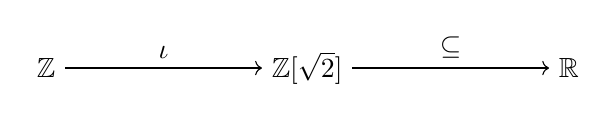
\begin{tikzpicture}[node distance=2.5cm]
\node (Z) {$\mathbb{Z}$};
\node[right=of Z] (Zsqrt) {$\mathbb{Z}[\sqrt2]$};
\node[right=of Zsqrt] (R) {$\mathbb{R}$};
\draw[->] (Z) -- node[above] {$\iota$} (Zsqrt);
\draw[->] (Zsqrt) -- node[above] {$\subseteq$} (R);
\end{tikzpicture}
\end{center}

埋め込み $\iota$ は環準同型であり、像が $\mathbb{Z}[\sqrt{2}]$。Lean 証明ではこれらの構造が陰に利用されている。

\section*{結語}
上記 5 問は、直積・商・多項式・行列・部分環という基本的な環構成を、射や普遍性を通じて理解させるものである。CODEX (OpenAI) による Lean 実装 (`S7.lean`) と本資料は互いに補完し合う形で用いていただきたい。

\end{document}
